% HI ionizations per primary particle in the z = 10 IGM.
% PRESCRIPTION: igm_losses.py (the loss routes and E). The deposition-fit route
% (models A/B/C) is OBSOLETE and is retained only as the cross-check.
% Numbers reproduced by:  python3 yield_comparison.py
% Figure:  python3 ionization_yield_igm.py
% Gate: python3 check_provenance.py ionization_yield.tex \
%              yield_comparison_results.json ionization_yield.log
\documentclass[11pt,a4paper]{article}
\usepackage[margin=2.4cm]{geometry}
\usepackage{amsmath,amssymb,booktabs,graphicx,xcolor}
% Figures live in Images/ since the 2026-09-15 reorganisation. Both entries
% are listed so the document builds either from Text_files/ or from the root.
\graphicspath{{../Images/}{Images/}{./}}

\usepackage[colorlinks=true,linkcolor=black,citecolor=black,urlcolor=blue]{hyperref}
\usepackage{siunitx}
\DeclareSIUnit{\erg}{erg}
\newcommand{\ion}[2]{\textsc{#1\,\MakeLowercase{#2}}}
\newif\ifprovdraft
\provdrafttrue
\newcommand{\src}[1]{%
  \ifprovdraft
    \ifmmode{}^{\text{\color{gray}\scriptsize\texttt{#1}}}%
    \else{\color{gray}\scriptsize$^{\texttt{#1}}$}%
    \fi
  \fi}

\title{Average number of HI ionizations per primary particle\\
\large Intergalactic medium at $z=10$, $x_e = 10^{-4}$\\
\large Computed from the \texttt{igm\_losses} energy-loss prescription}
\author{Generated with an AI assistant, under the project Master Rules}
\date{Reproduced by \texttt{python3 yield\_comparison.py}}

\begin{document}
\maketitle

\begin{abstract}
\noindent
We compute the mean number of \ion{H}{i} ionizations produced by one primary
electron ($10^{2}$--$10^{12}$~eV) or photon ($10^{1}$--$10^{5}$~eV) in the
neutral IGM at $z=10$ with a static ionized fraction $x_e = 10^{-4}$, counting
every ionization anywhere in the cascade. \textbf{Electron propagation is
computed with \texttt{igm\_losses.py}}: seven competing loss mechanisms
(adiabatic expansion, synchrotron, inverse Compton with the Klein--Nishina
kernel, Coulomb, collisional excitation, collisional ionization,
bremsstrahlung), with ionizations counted event by event against the RBED cross
section of Kim et al.~\cite{kim00} and knock-on electrons followed explicitly
through the BED singly-differential cross section of Kim \&
Rudd~\cite{kimrudd94}. Discarding the energy inverse Compton gives to the CMB
(\textbf{the loss route}) the yield saturates at
$1.171\times10^{4}$\src{N\_e\_loss\_sat} ion pairs. Following the upscattered CMB
photons that are reabsorbed (\textbf{the loss+IC route}) raises it to
$4.911\times10^{6}$\src{N\_e\_loss\_ic\_sat}, a factor
$419.5$\src{lossic\_over\_loss\_sat}. The deposition-fraction route used in earlier
versions of this document (models A/B/C, built on the Shull \& van Steenberg
fit) is \textbf{obsolete}; it survives only as the independent cross-check that
validated this one, agreeing to
$1.071$\src{lossic\_over\_depfit\_1e12} at saturation and to
$1.017$\src{loss\_over\_ic\_min}--$1.102$\src{loss\_over\_ic\_max} below 1~MeV.
\end{abstract}

\section{Assumptions}
\begin{enumerate}\itemsep2pt
\item \textbf{Target}: neutral hydrogen of the IGM at $z=10$, number density
      $n_{\rm HI} = \SI{2.5287e-4}{\per\cubic\centi\metre}$\src{n\_H\_cm3\_route2},
      ionized fraction $x_e = 10^{-4}$\src{x\_e\_route2} held static.
\item \textbf{Ionization threshold} $E_{\rm th} = \SI{13.5984}{\electronvolt}$\src{E\_th\_eV\_route2}
      (one Rydberg, as \texttt{igm\_losses} defines it).
\item \textbf{Magnetic field} $B_0 = \SI{1e-13}{\tesla}$\src{B0\_T\_route2}
      comoving (1~nG), giving $U_B/U_{\rm CMB}\sim10^{-7}$ at $z=10$ --- which
      is why synchrotron is negligible rather than assumed away.
\item \textbf{Expansion} at $H(z) = \SI{4.4717e-17}{\per\second}$\src{H\_z\_s\_route2}
      (Planck18, the cosmology \texttt{igm\_losses} itself uses).
\item \textbf{Cascade}: knock-on electrons are followed explicitly. The
      secondary energy is drawn from the BED SDCS~\cite{kimrudd94}, not from a
      deposition fraction.
\item \textbf{One generation} of IC-secondary photons --- derived, and exactly,
      in \S\ref{sec:closure}.
\item \textbf{Environmental parameters are adjustable} through
      \texttt{igm\_config.py}; every value above is what the run actually used.
\end{enumerate}

\section{Method}
An electron of kinetic energy $K$ loses energy through seven channels; only the
collisional-ionization channel makes ion pairs, and it makes them one at a time:
\begin{equation}
\boxed{\;Y(K) = \int_{E_{\rm th}}^{K} R(K')\,
   \bigl[\,1 + \langle Y(\varepsilon)\rangle_{p(\varepsilon|K')}\,\bigr]\,dK',
 \qquad R(K') = \frac{n_{\rm HI}\,v(K')\,\sigma_{\rm ion}(K')}{L_{\rm total}(K')}\;}
\label{eq:D}
\end{equation}
$R$ is the number of ionization events bought per eV given up, with every
competing channel in the denominator; $p(\varepsilon|K')$ is the BED secondary
spectrum. Equation~\eqref{eq:D} is \textbf{the loss route}. The energy handed to the
CMB is discarded there; \textbf{the loss+IC route} follows it,
\begin{equation}
\boxed{\;Y_E(K) = Y_D(K) + \int_0^{K}
  \frac{L_{\rm IC}}{L_{\rm tot}}(K')\; G(\gamma(K'))\, dK'\;}
\label{eq:E}
\end{equation}
with $G$ the ionizations per eV radiated, obtained by folding the
Blumenthal \& Gould~\cite{bg70} scattered-photon spectrum against the absorption
probability and the photon yield. The IC branching ratio is the
Klein--Nishina-corrected one from \texttt{igm\_losses}; the photoelectron
released by an absorbed secondary cascades with $Y_D$, not with a fit.

\paragraph{Why mixing a KN loss rate with a Thomson-limit photon spectrum is
legitimate.} Checked, not assumed, at the energies that actually deliver the
ionizations: at 5\,\% of the channel
($K = \SI{2.0224e7}{\electronvolt}$\src{Ewindow\_lo\_eV}) the KN factor is
$1.0$\src{FKN\_window\_lo}; at 95\,\%
($K = \SI{3.5541e8}{\electronvolt}$\src{Ewindow\_hi\_eV}) it is
$0.9999$\src{FKN\_window\_hi}. Corrections stay below $10^{-4}$ across the
window.

\subsection{Why one generation suffices}\label{sec:closure}
Every absorbed secondary photon has $\varepsilon_1 \lesssim \SI{1218}{\electronvolt}$,
so its photoelectron has $\gamma = 1.0024$; reaching \SI{13.6}{\electronvolt}
from there would need a seed photon of $1310\,kT$, Planck occupancy
$\sim10^{-569}$. On the tracked spectrum $G(\gamma)=0$ identically.

\section{The loss budget}
\begin{table}[h]\centering\small
\begin{tabular}{@{}lrr@{}}
\toprule
mechanism & peak fraction of $dK/dt$ & at $K$ [eV] \\
\midrule
inverse Compton (KN)  & $1.000$\src{peakfrac\_compton} & $\ge10^{9}$ \\
collisional ionization & $0.7304$\src{peakfrac\_ionization} & $\sim5\times10^{3}$ \\
collisional excitation & $0.3532$\src{peakfrac\_excitation} & $10^{2}$ \\
adiabatic expansion    & $0.0929$\src{peakfrac\_adiabatic} & $\SI{3.046e5}{}$\src{peakE\_adiabatic\_eV} \\
Coulomb                & $0.002336$\src{peakfrac\_coulomb} & --- \\
bremsstrahlung         & $4.159\times10^{-5}$\src{peakfrac\_bremsstrahlung} & --- \\
synchrotron            & $1.176\times10^{-7}$\src{peakfrac\_synchrotron} & --- \\
\bottomrule
\end{tabular}
\end{table}

\noindent
\textbf{Adiabatic expansion reaches $9.2\%$} and has no counterpart in the
obsolete route, which had no expansion term at all. The last three channels stay
below a quarter of a per cent everywhere --- which is the quantitative reason the
old two-channel treatment could ignore them and still land within 10\,\%.

\section{Result}
\begin{figure}[h]\centering
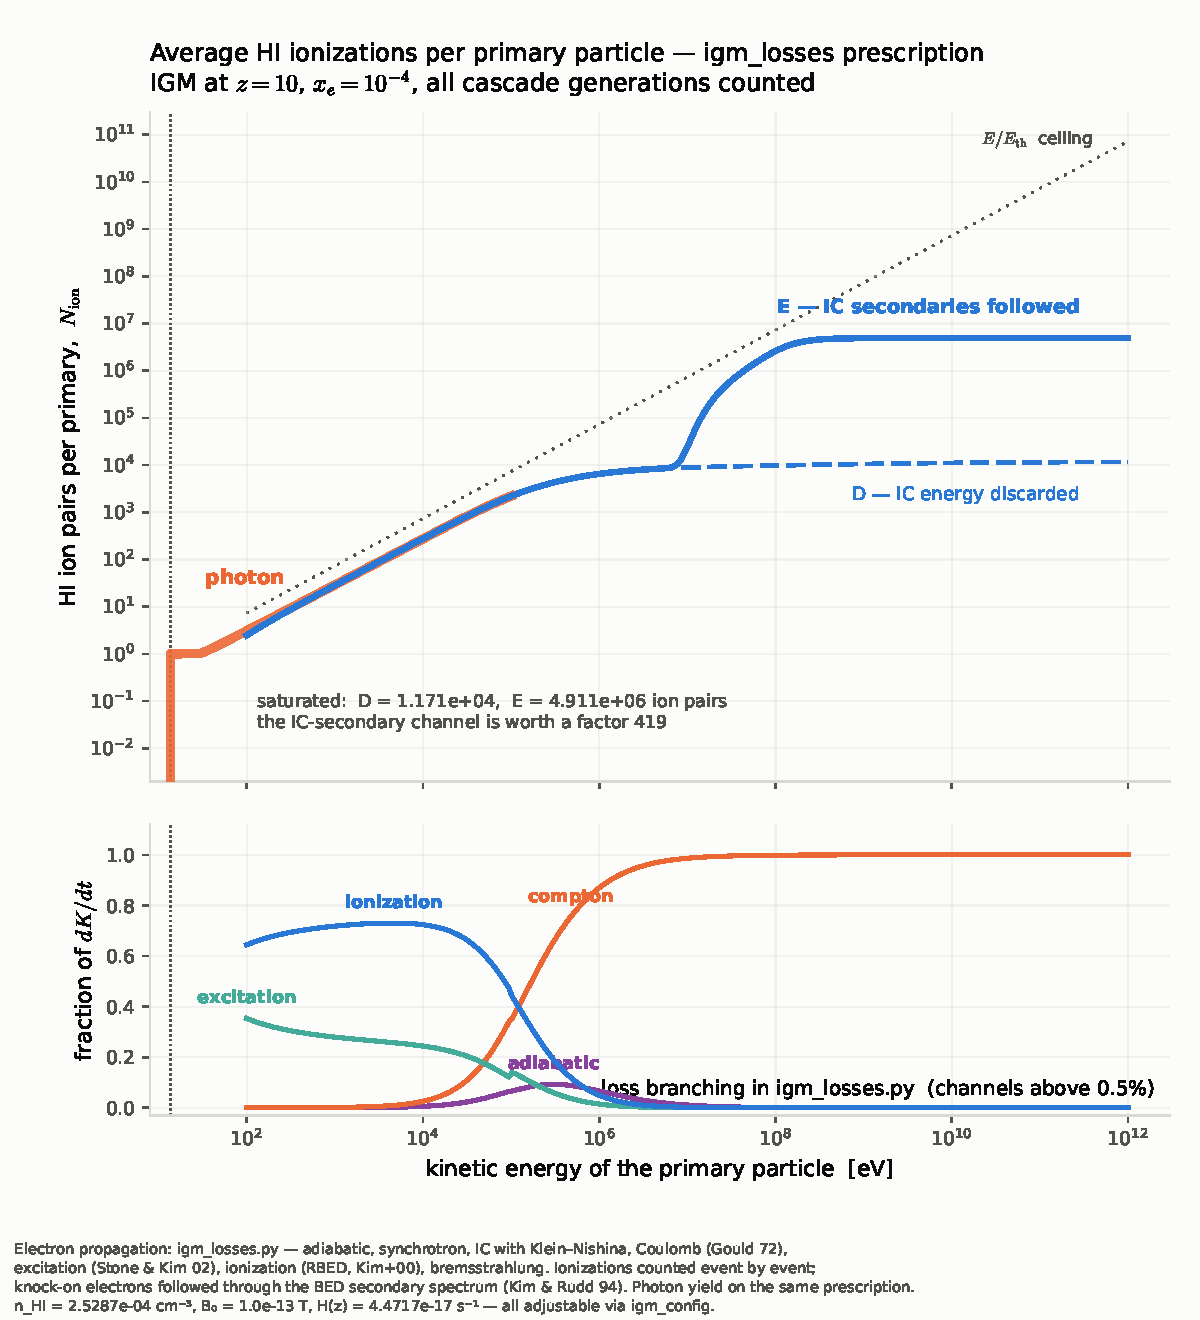
\includegraphics[width=0.80\textwidth]{ionization_yield_fig_igm.pdf}
\caption{\ion{H}{i} ion pairs per primary against primary kinetic energy, on the
\texttt{igm\_losses} prescription. \emph{Upper:} the loss route (IC energy discarded)
and the loss+IC route (IC secondaries followed), with the photon curve on the same
prescription and the $E/E_{\rm th}$ ceiling. \emph{Lower:} the seven-channel loss
branching that produces the shape. Produced by
\texttt{ionization\_yield\_igm.py}.}
\end{figure}

\begin{table}[h]\centering\small
\caption{$N_{\rm ion}$ per primary. The loss+IC route is the answer; D is shown to isolate
the IC-secondary channel.}
\begin{tabular}{@{}rrrr@{}}
\toprule
$K$ [eV] & $e^-$ (D) & $e^-$ (E) & $W = K/N$ [eV] \\
\midrule
$10^{2}$  & $2.477$\src{N\_e\_loss\_1e+02} & $2.478$\src{N\_e\_loss\_ic\_1e+02} & $40.37$\src{W\_loss\_1e+02} \\
$10^{3}$  & $28.35$\src{N\_e\_loss\_1e+03} & $28.36$\src{N\_e\_loss\_ic\_1e+03} & $35.27$\src{W\_loss\_1e+03} \\
$10^{4}$  & --- & --- & $36.18$\src{W\_loss\_1e+04} \\
$10^{5}$  & --- & --- & $45.4$\src{W\_loss\_1e+05} \\
$10^{6}$  & $6523$\src{N\_e\_loss\_1e+06} & $6523$\src{N\_e\_loss\_ic\_1e+06} & --- \\
$10^{9}$  & $1.058\times10^{4}$\src{N\_e\_loss\_1e+09} & $4.892\times10^{6}$\src{N\_e\_loss\_ic\_1e+09} & --- \\
$10^{12}$ & $1.171\times10^{4}$\src{N\_e\_loss\_1e+12} & $4.911\times10^{6}$\src{N\_e\_loss\_ic\_1e+12} & --- \\
\bottomrule
\end{tabular}
\end{table}

\begin{itemize}\itemsep1pt
\item $W$ is \emph{not} a constant: $\SI{40.37}{\electronvolt}$\src{W\_loss\_1e+02}
      at $10^2$~eV, $\SI{35.27}{\electronvolt}$\src{W\_loss\_1e+03} at $10^3$~eV,
      $\SI{45.40}{\electronvolt}$\src{W\_loss\_1e+05} at $10^5$~eV, where IC has
      begun to take the energy away.
\item $E_{\rm crit} = \SI{1.4866e5}{\electronvolt}$\src{E\_crit\_D\_eV}, where
      Compton overtakes excitation plus ionization.
\item Photon primaries: $N_\gamma = 3.077$\src{N\_gamma\_loss\_1e+02} at $10^2$~eV
      and $28.97$\src{N\_gamma\_loss\_1e+03} at $10^3$~eV --- one ionization plus
      the photoelectron's cascade, on the same prescription.
\end{itemize}

\section{Validation against the obsolete route}
The deposition-fraction route (models A/B/C; Shull \& van
Steenberg~\cite{svds} via the Ricotti fit reproduced in Furlanetto \&
Stoever~\cite{fs10}) shares nothing with this one but the physical scenario. It
is retained for exactly one purpose:
\begin{itemize}\itemsep1pt
\item below 1~MeV, D/B lies between $1.017$\src{loss\_over\_ic\_min} and
      $1.102$\src{loss\_over\_ic\_max};
\item at $10^{12}$~eV, D/B $= 1.32$\src{loss\_over\_ic\_1e12}, and the excess is
      Klein--Nishina: the obsolete route used the Thomson limit, where the KN
      factor is $0.8111$\src{F\_KN\_at\_1e12} at that energy;
\item with the secondary channel on both sides, E/C $= 1.071$\src{lossic\_over\_depfit\_1e12}.
\end{itemize}
The two environments have since been \emph{harmonised} on the route-1 values,
at the user's instruction: $n_{\rm H}$ now differs by
$1.05\times10^{-10}$\src{env\_dn\_H}, i.e.\ floating-point round-off, and the
ionization threshold agrees exactly, $\Delta E_{\rm th} = 0$\src{env\_dE\_th}
--- \texttt{igm\_losses.py} was moved from one Rydberg to the NIST binding
energy. Any residual disagreement between the routes is therefore method, not
input. One input is \emph{not} harmonised and is reported rather than hidden:
$H(z)$, which the two routes evaluate from the same Planck 18 cosmology by
different code paths, differing by $0.001369$\src{env\_dH\_z}. It reaches the
yield only through the adiabatic loss term.

\section{What was \emph{not} checked}
\begin{enumerate}\itemsep2pt
\item \textbf{No independent reimplementation} of \texttt{igm\_losses} itself.
      The agreement above is with the obsolete route, which is a genuinely
      separate construction, but both were written in this project.
\item \textbf{Helium} is absent from the target in both routes.
\item \textbf{$x_e$ is static}; no back-reaction of the cascade on the gas.
\item \textbf{Cosmological transport of the primary} is not modelled: ``per
      primary'' presupposes an interaction.
\item \textbf{A fixed-$z$ snapshot.} \texttt{igm\_losses} is built to integrate
      trajectories over cosmic time; here it is evaluated at $z=10$ throughout.
      Following a real electron as it redshifts would change the adiabatic and
      IC terms.
\end{enumerate}

\paragraph{Reproducibility.} Deterministic; no random numbers. Run
\texttt{python3 yield\_comparison.py} for the registry and
\texttt{python3 ionization\_yield\_igm.py} for the figure, then
\texttt{python3 check\_provenance.py ionization\_yield.tex
yield\_comparison\_results.json ionization\_yield.log}.

\begin{thebibliography}{9}\small
\bibitem{kim00} Y.-K. Kim, J.~P. Santos \& F. Parente, \emph{Phys. Rev. A} \textbf{62},
  052710 (2000). RBED ionization cross section, their eq.~(20) --- NOT the RBEB
  of their eq.~(22); verified against the code in \texttt{photon\_vs\_electron.pdf}
  \S\,''Audit against the sources''. \emph{In the tree}:
  \texttt{papers/PhysRevA.62.052710-kim-santos-parente-2000-rbed.pdf}.
\bibitem{kimrudd94} Y.-K. Kim \& M.~E. Rudd, \emph{Phys. Rev. A} \textbf{50}, 3954 (1994).
  \emph{In the tree}: \texttt{papers/PhysRevA.50.3954-kim-rudd-1994-bed.pdf}.
  BED singly-differential cross section (the real Table~I $\mathrm{d}f/\mathrm{d}w$,
  not the $N/(1+w)^2$ of BEB); the secondary-electron spectrum.
\bibitem{stonekim02} P.~M. Stone \& Y.-K. Kim, \emph{J. Phys. B} \textbf{35}, 1675 (2002).
  Collisional excitation of H.
\bibitem{gould72} R.~J. Gould, \emph{Physica} \textbf{60}, 145 (1972). Coulomb losses.
\bibitem{bg70} G.~R. Blumenthal \& R.~J. Gould, \emph{Rev.\ Mod.\ Phys.} \textbf{42}, 237
  (1970). Inverse Compton and bremsstrahlung; eq.~(2.42) for the scattered spectrum.
\bibitem{planck18} Planck Collaboration, \emph{A\&A} \textbf{641}, A6 (2020).
\bibitem{svds} J.~M. Shull \& M.~E. van Steenberg, \emph{ApJ} \textbf{298}, 268 (1985).
  \emph{Obsolete route only.}
\bibitem{fs10} S.~R. Furlanetto \& S.~J. Stoever, \emph{MNRAS} \textbf{404}, 1869 (2010).
  \emph{In the tree}; eqs.~(2), (13), (14). \emph{Obsolete route only.}
\end{thebibliography}
\end{document}
